\documentclass[12pt, a4paper]{article}
%\usepackage{natbib}
\usepackage{cite}
\usepackage{amsmath,amssymb,amsfonts}
\usepackage{algorithmic}
\usepackage{graphicx}
\usepackage{textcomp}
\usepackage{xcolor}
\usepackage[inkscapeformat=pdf]{svg}
\usepackage[inline]{enumitem}
\usepackage[hidelinks]{hyperref}

\usepackage{myacronyms}
\usepackage{listings}
\usepackage{todonotes}
\newcommand{\note}[3]{\todo[inline,linecolor=#1,backgroundcolor=#1!25,bordercolor=#1]{\textbf{#2:} #3}}
\newcommand{\angela}[1]{\note{blue}{Angela}{#1}}

\newenvironment{inlinelist}{\begin{enumerate*}[label=\emph{(\roman*)}]}{\end{enumerate*}}

\usepackage{cleveref}

\begin{document}

\title{Towards collective operating systems through Aggregate Computing}

\author{Angela Cortecchia}
\date{\today}
\maketitle


% ----------------------------------------
\section{State of the art}
\label{sec:state-of-the-art}

\sloppypar
\paragraph{Collective Adaptive Systems and Macroprogramming.}
\acp{cas} are systems composed of multiple autonomous entities,
including devices, sensors, and actuators, which interact locally to achieve a global goal~\cite{ferscha2015}.
%
\acp{cas} are designed to adapt to dynamic changes in the environment, system requirements, or operational conditions.
%These systems are designed to adapt to dynamic changes in the environment, system requirements, or operational conditions.
%
\ac{cas} are commonly employed in \ac{cps} applications where devices collaborate to monitor and control a
physical environment or to provide services to users.

Managing a single device in a distributed system presents several challenges,
such as \textbf{scalability}, \textbf{device heterogeneity},
\textbf{resource constraints}, and the need to adapt to \textbf{dynamic changes}.
%
Recent techniques promote the usage of \emph{collective} abstractions at the programming level
(\emph{macroprogramming}~\cite{casadei22}) to address these challenges while achieving
\begin{inlinelist}
    \item distributed intelligence,
    \item resource pooling,
    \item adaptability, and
    \item robustness.
\end{inlinelist}
%
In macroprogramming, the behavior of a system is expressed macroscopically through a single program,
hiding the complexity of individual component interactions under the hood.
%
The approach has been successfully applied, among others, to
\ac{wsn}~\cite{1440891},
\ac{iot} applications~\cite{noor19,mizzi18}
and
swarm robotics~\cite{buzz}.

\sloppypar
\paragraph{Self-organization and Field Calculus.}

Tackling environmental changes, coordinating many agents effectively, and maintaining resilience
in face of unpredicted events promote approaches based on \emph{self-organization}.
%
In them,
interaction among multiple independent and autonomous software entities drives the evolution of the overall system.
%
Over time,
various approaches emerged based on tuple spaces,
such as \textit{$\sigma\tau-$Linda}~\cite{ViroliCoordination2012} and \textit{MARS}~\cite{mars},
in which the coordination is mediated by a shared memory space.
%
In parallel,
other approaches relied on \emph{computational fields},
distributed data structures mapping space and time to values,
to coordinate interactions among agents.
%
Notable examples are \emph{\ac{tota}}~\cite{tota} and \emph{co-fields}~\cite{MameiZL04},
a tuple-based middleware
for field-based coordination.
%
These seminal works laid the foundation for the development of \ac{fc}~\cite{JLAMP2019},
a foundational model~\cite{TOCL2019} for the field-based coordination of distributed systems.
%
The \ac{fc} captures field coordination through composable functions
combining fields, and supporting the definition of their behavior in time
and (local) space through views of field values in the neighborhood.
%
%\ac{fc} specifies system behavior through a dynamic network of directly communicating devices,
%using functional compositions of operators to manipulate computational fields.
%
In \ac{fc}, devices execute asynchronous computational rounds with three phases:
\begin{inlinelist}
    \item \emph{context building},
    \item \emph{program execution}, and
    \item \emph{export sharing}.
\end{inlinelist}
%
%Globally,
%\ac{fc} aligns individual device behavior with the network's overarching behavior,
%specifying mappings for each device's computation round at space-time events.

\sloppypar
\paragraph{Aggregate Computing/Programming.}
\ac{ap} (or \ac{ac})~\cite{BealIEEEComputer2015} is a functional macroprogramming approach for the compositional development
of self-adaptive \ac{iot} services,
based on the abstractions of \ac{fc}.

\ac{ac} programs the behavior of distributed systems by defining interactions among devices as a whole,
shifting the computation unit from individual devices to collaborative groups.
%
This approach supports the specification, analysis, simulation,
and runtime execution of collective services across diverse IoT architectures~\cite{FI2020-pulverization}.
%
The paradigm embodies three key traits:
\begin{inlinelist}
    \item \emph{global stance with global-to-local mapping}, targeting the entire distributed IoT ecosystem,
    \item \emph{service compositionality}, describing rich collective services through functional composition, and
    \item \emph{abstraction}, enabling adaptivity by abstracting from low-level details.
\end{inlinelist}
%
These traits facilitate concise articulation of complex solutions in the design phase and provide flexibility in execution and deployment strategies during operation.
%
Each device locally evaluates the program at a set frequency and communicates with neighboring devices as needed.

\sloppypar
\paragraph{Aggregate Processes.}
\label{par:aggregate-processes}

A system has been developed to manage \emph{aggregate processes}~\cite{aggregate-processes} based on \ac{fc}
to address the challenges of managing multiple concurrent aggregate operations in a distributed environment.

Aggregate processes are concurrent field computations sustained by a dynamic team of devices,
with their spatial region opportunistically changing over time.
%
This concept captures aggregate behavior, dynamicity, context orientation, and intrinsic resiliency.
%
It offers benefits such as limiting computational resource consumption, maintaining quality of service,
and enhancing distributed computation dynamics.
%
While similar to concentrated processes,
aggregate processes allow multiple computations to overlap in both space and time,
they currently do not consider issues related to permissions, signals, or interprocess communication.

\sloppypar
\paragraph{Tools for Aggregate Computing.}
Various tools have been developed to support the \ac{ac} paradigm,
each tailored to specific characteristics and target devices.

\emph{ScaFi (Scala Fields)}~\cite{scafi} is a Scala-based framework providing a \ac{dsl}, libraries,
a simulation environment with a GUI integrated with the Alchemist simulator~\cite{PianiniJOS2013},
and an actor-based runtime for aggregate computing systems.
%
ScaFi runs aggregate programs on the \ac{jvm} and in web browsers through the ScaFi Web tool~\cite{Coordination2021-scafiweb}, for rapid prototyping.

\emph{Protelis}~\cite{PianiniSAC2015} is a functional programming language implementing a higher-order version of \ac{fc},
with a C-like syntax for building reusable components of aggregate systems.
%
It provides domain-specific APIs interoperable with Java through Protelis-Lang~\cite{SASO2017-protelislang}, but requires a \ac{jvm} to run.

\emph{FCPP}~\cite{DBLP:journals/scp/AudritoT24} is a C++ library implementing FC for simulations of distributed systems.
%
It supports running aggregate programs on low computational capacity devices but has a less ergonomic syntax.

\emph{Collektive} is a prototype \ac{dsl} extending \ac{fc} with \ac{xc}~\cite{AudritoCDSV24},
offering a more expressive language with a user-friendly syntax compared to FCPP and Protelis.
%
It is natively multi-platform, allowing development on various devices.

\sloppypar
\paragraph{Distributed Operating Systems.}
A \ac{dos}~\cite{dos} coordinates and manages resources across independent networked computational nodes,
each holding a specific subset of the global operating system.
%
It presents a unified system to the user,
akin to a centralized \ac{os}, ensuring transparency, reliability, and efficiency despite resource distribution complexity.
%
%The kernel at each node provides essential services such as process and memory management.
%
Architecturally,
a \ac{dos} must balance individual and overall system goals,
requiring a design approach that separates policy from mechanism.
%
Its functioning relies on multi-level collaboration among system components,
each node has \emph{part} of the distributed resources, and the system distributes the different processes to execute among the nodes,
while the user perceives the system as a single entity.

\subsection{Coherence with my previous experiences}
\label{subsec:coherence-with-the-educational-path}
The proposed research project extends my Master’s degree final year and thesis activities.
%
During my Master’s studies, exploration of  \ac{fc} and \ac{ac} began in the “Pervasive Computing” course.
%
My project's colleagues and I developed a Rust-based reimplementation of aggregate computing's core engine,
alongside a Scala 3 version, providing a solid foundation in \ac{fc} and \ac{ac}.

My Master’s thesis focused on expanding the Collektive DSL by integrating constructs from the \ac{xc} calculus,
demonstrating its potential for \ac{ac} applications through a prototype tested on simple case studies.

During the development of the Master's degree,
I had the opportunity to apply for a research grant that was awarded to me from the \emph{Consortium GARR}~\footnote{\url{https://www.garr.it/it/}},
the Italian ``Group for Research Networks Harmonisation'',
ongoing work extends the Collektive DSL by creating a standard library of functions for \ac{ac} application development and showcasing language functionalities through demos.

These experiences facilitated collaborations with various researchers, including a collaboration with Professor Sven Tomforde from
the University of Kiel,
on managing communication between maritime autonomous surface ships.

Furthermore,
the work done has allowed me to paper submissions to the \emph{IEEE International Conference on Autonomic Computing and Self-Organizing Systems} (ACSOS 2024),
and the \emph{International Symposium on Distributed Simulation and Real Time Applications} (DS-RT 2024),
focusing on generalizing the \emph{Vascular Morphogenesis Controller} (VMC)~\cite{ZahadatHS17} algorithm using the \ac{ac} paradigm
and developing an architecture and prototype for monitoring distributed simulations of distributed systems using Collektive.

% ----------------------------------------
\section{Project description}
\label{sec:project-description}

%\sloppypar
\subsection{Motivation.}
\label{subsec:motivation.}

Typical applications of aggregate computing run a single, complex algorithm.
%
However,
there are scenarios where these algorithms need to be added, removed,
or manipulated at runtime without affecting others.
%
For example, in crowd management,
law enforcement might need to alter the movement of a portion of the crowd to prevent congestion.
%
This parallels how modern \acp{os} manage processes but extends to space and time.
%
To achieve similar functionalities in aggregate computing,
it is necessary to advance towards the development of \emph{\ac{cos}}.
%
These systems handle concerns similar to traditional \acp{os} --such as managing devices, users, groups, permissions, and signals--
but in a distributed environment where these concepts involve space and time.
%
Additionally,
collective systems often consist of heterogeneous devices,
requiring the system to abstract their differences while managing their specificities.

\subsection{Idea}
\label{subsec:idea}

\begin{figure}
    \centering
    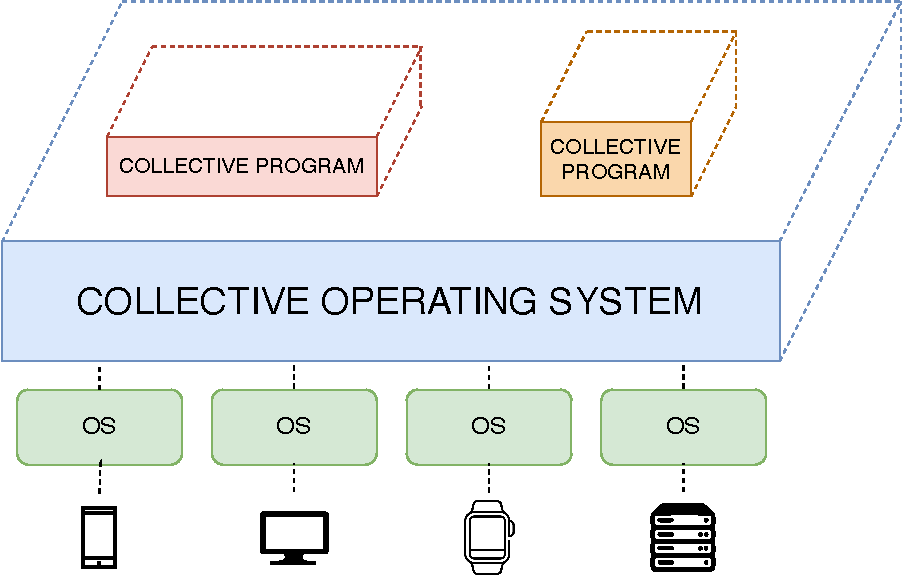
\includegraphics[width=0.8\textwidth]{figures/system}
    \caption{
        High-level view of the system.
        The collective operating system is seen as a middleware that manages the different aggregate programs and the devices
        of different types.
    }\label{fig:system}
\end{figure}

\begin{figure}[h!]
    \centering
    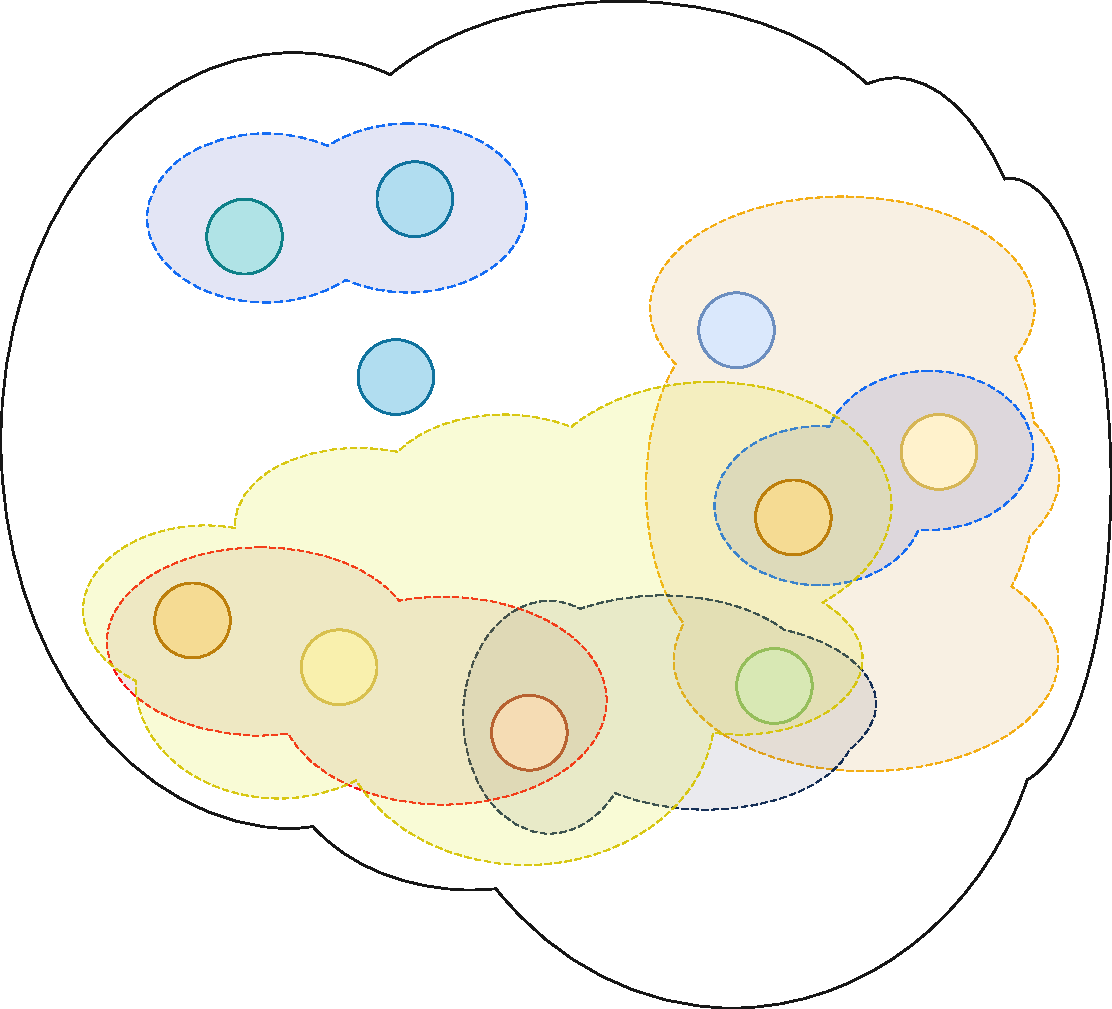
\includegraphics[width=0.6\textwidth]{figures/processes}
    \caption{
        Aggregate processes executed on a collective operating system.
        Solid circumferences represent devices, their internal color indicates the device kind
        (same color, same kind).
        The space delimited by the solid black line indicates the region of the space where the
        \ac{os} is active.
        Dashed zones are aggregate processes,
        the same color indicates the same process.
        Notice that devices may participate in one, none, or multiple processes.
        Also, differently than the current proposal for aggregate processes,
        with the proposed approaches the same process can be non-contiguous in space-time.
    }\label{fig:processes}
\end{figure}

The general idea of the project is conveyed graphically by
\Cref{fig:system} and \Cref{fig:processes}.
%
\Cref{fig:system} shows a high-level view of the system,
where the \ac{cos} works as middleware between the different aggregate programs and the devices where they run.
%
From another perspective,
\Cref{fig:processes} shows aggregate processes that execute over the shared \ac{os},
involving different sub-portions of the space-time.
%
Each process can be executed on different devices and a device can execute different processes,
so it is possible to have an overlap of processes on the devices.
%
Note that, differently than the current aggregate processes~\cite{EAAI2020-processes},
through the proposed approach the shared \ac{os} permits processes which are non-contiguous in space.

Differently from the \ac{dos},
the \ac{cos} is situated and can manage multiple aggregate processes executed on many devices,
with the aim of evaluating the processes as a collective distributed across space and time.

\subsection{Research goals and challenges}
\label{subsec:research-goals-and-challenges}

Realizing such a system requires an understanding of the meaning of various concepts when they are tied to space and time.

\paragraph{Users and permissions.}
\label{par:users-and-permissions}
In classic \acp{os},
exists the concept of users and groups,
with access to resources and services based on their roles and context.
%
However,
in aggregate or collective systems,
there is currently no clear definition of users or groups and how to manage their permissions.
%
For example,
in crowd management,
there are different user types:
the crowd and the law enforcement officers managing them.
%
Law enforcement officers have more permissions and can execute different actions compared to the crowd.

\paragraph{Signals and interrupts.}
\label{par:signals-and-interrupts}
The concept of interrupts and signals requires careful consideration in the context of aggregate systems.
%
Similar to permissions,
it's crucial to identify the sender of a signal,
as it can alter the behavior of the recipient process.
%
In aggregate environments,
the management of signals is closely linked to permissions,
ensuring that only authorized entities can send specific signals to target processes without affecting others.
%
Understanding the implications of signals like pause, continue, or terminate is essential,
as termination in aggregate processes is collectively managed and typically cannot be interrupted.
%
However,
exceptions may arise where individual devices initiate process termination or when a process loses access to shared resources,
posing distributed consensus challenges.
%
For instance, in crowd management scenarios,
third-party entities may intervene by interrupting crowd management processes based on crowd sensing or steering observations.
%
This highlights the necessity of a runtime mechanism to facilitate dynamic changes in system behavior.

\paragraph{Intra-process communication.}
\label{par:intra-process-communication}
Communication between processes in different spatial regions is another challenge.
%
For instance,
in a crowd steering and tracking scenario,
processes managing these tasks need to communicate to effectively manage the crowd.
%
A steering process must communicate with a tracking process to understand crowd locations and direct movement accordingly.

This type of communication,
typically managed by shared memory spaces or files in traditional systems,
isn't directly applicable in distributed processes,
requiring further research.
%
Currently, aggregate processes lack this communication capability.

\paragraph{Distributed sensors and actuators.}
\label{par:distributed-sensors-and-actuators}
Managing distributed sensors and actuators presents another challenge.
%
By combining multiple devices into a single entity or logical resource,
we can achieve a higher-level programming approach and involve heterogeneous devices as a ``collective sensor'',
realizing a ``sensor fusion''~\cite{sasiadek2002sensor} at the application level.
%
In crowd management,
various sensors observe the crowd and send data to the system,
which should treat the data as coming from a single entity for more abstract and efficient management.
\\

The proposed research project therefore aims to investigate the development of \emph{\ac{cos}},
based on the \ac{ac} paradigm,
offering consistency and resilience to failures,
while adapting to \emph{dynamic} changes in the environment.
%%
%The paradigm itself of \ac{ac} also offers consistency and resilience to failures,
%and the possibility to adapt to \emph{dynamic} changes in the environment.

\subsection{Reference scenarios}
\label{subsec:example-applications}

\sloppypar
\paragraph{Crowd management.}

The system's versatility extends to various scenarios,
including crowd management and surveillance.
%
It can effectively manage crowd movement to prevent congestion and hazardous situations by sensing and steering crowds.
%
Drones or sensors running aggregate processes observe and send data to the system,
treating them as a collective entity (distributed sensors and actuators).
%
Crowd movement is directed based on data evaluation,
with communication between processes facilitating efficient crowd management.
%
Intra-process communication ensures coordination between processes, enabling an effective crowd direction based on the situation.
%
Law enforcement intervention may be necessary,
involving signal or interrupt transmission to alter the crowd direction.

\sloppypar
\paragraph{Autonomous navigation.}
In the collaboration with Prof. Sven Tomforde,
a key challenge that has been presented involves communication between maritime autonomous surface ships in the Kiel Canal.
%
These ships utilize varying communication technologies depending on their distance,
resulting in significantly different data rates.
%
For instance,
ships in closer proximity typically use 5G for communication and can exchange more data compared to those farther apart,
which rely on satellite communication.
%
It is believed that employing \ac{ac}, particularly through \ac{xc}, can address this issue.
%
The system should autonomously adapt to the most suitable communication technology,
prioritizing data exchange between ships to minimize communication errors.

\sloppypar
\paragraph{Smart cities.}
Many other application scenarios can be considered,
such as avoiding light pollution or traffic congestion in a smart city.
%
It could also be useful to manage the city's lighting based on the presence of people in the streets to avoid light pollution and save energy,
or to manage the traffic lights based on the presence of cars in the streets to avoid traffic congestion.

% ----------------------------------------
\section{Expected results}
\label{sec:expected-results}

As results of the proposed research project,
it is expected to bring
\begin{inlinelist}
    \item a contribution to the advancement of scientific and technological knowledge in the field of \ac{ac} and \ac{cas},
    \item a theoretical and executable model of the \ac{cos},
    \item a prototype of the system that is able to manage scenarios at least in a simulated environment,
    taking as reference scenarios the crowd management and the autonomous navigation scenarios mentioned in \Cref{subsec:example-applications}.
\end{inlinelist}

As a long-term vision,
the system will be able to manage many devices in a collective environment,
where the devices can be heterogeneous and can change over time.
%
Some of the application scenarios where the system can be used are
\begin{inlinelist}
    \item \emph{smart cities},
    \item \emph{swarm scenarios},
    \item \emph{crowd management},
    \item \emph{morphogenesis},
    \item \emph{autonomous vehicles},
    \item \emph{surveillance}.
\end{inlinelist}

% ----------------------------------------
\section{Subdivision of the project and timeline}
\label{sec:subdivision-of-the-project-and-timeline}

\begin{figure}
    \centering
    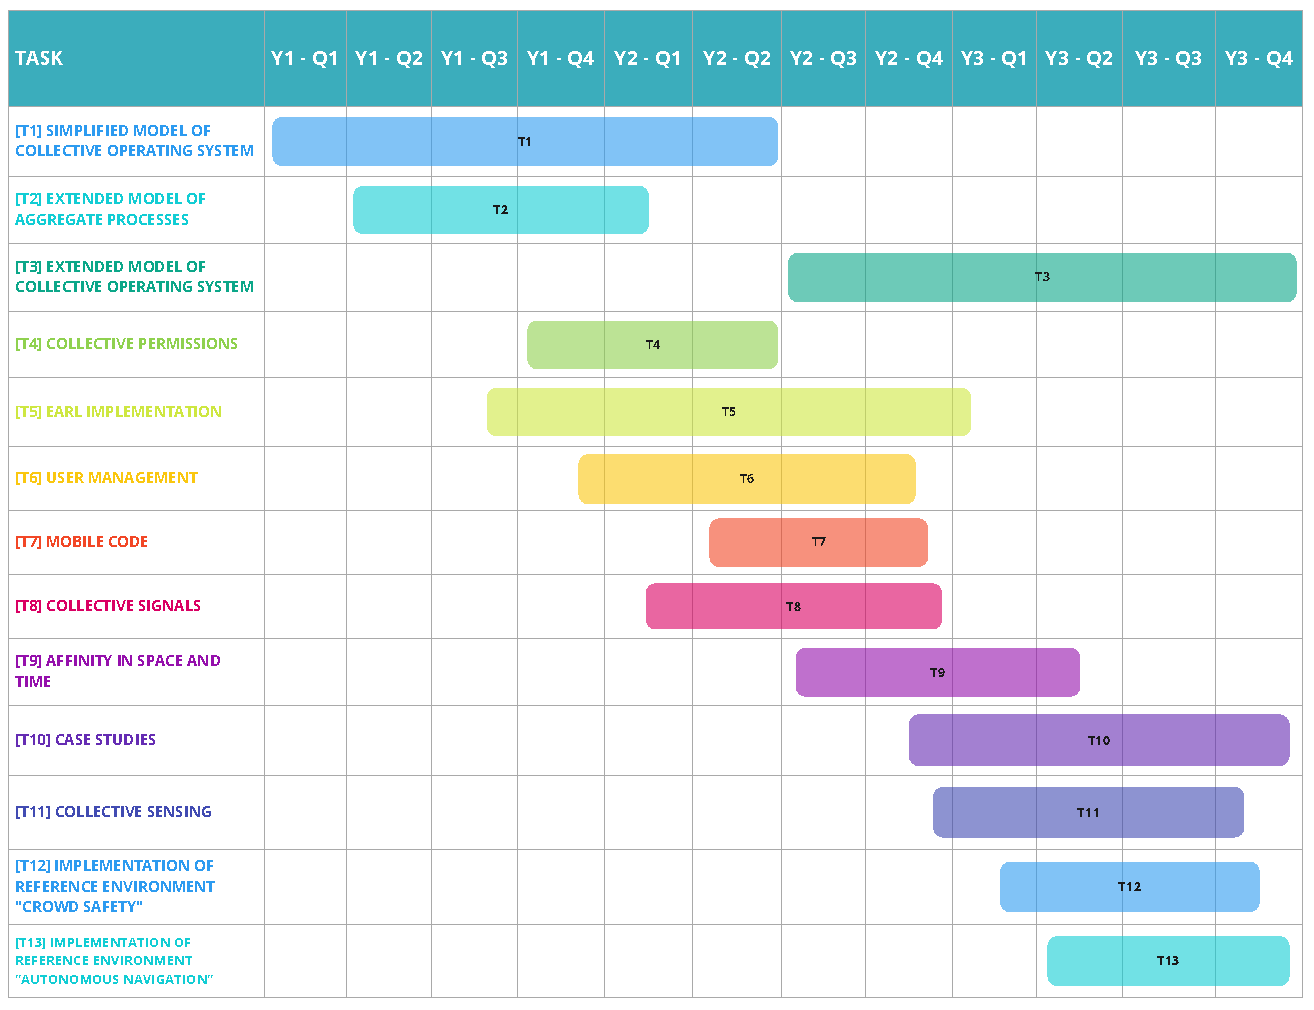
\includegraphics[width=0.99\textwidth]{figures/timeline}
    \caption{Hypothetical timeline of the three-year project.
        Years are subdivided in quarters, Q1 is from January to March,
        Q2 is from April to June, Q3 is from July to September, and Q4 is from October to December.
    }\label{fig:timeline}
\end{figure}

In the \Cref{fig:timeline} is shown a hypothetical timeline with tasks of the three years of the project,
where each year is subdivided into quarters.

\sloppypar
\paragraph{First year.}
In the project's first year,
a thorough exploration of the current state of the field is crucial,
along with establishing a simplified model for the new system.
%
This model will define key interconnected elements such as aggregate processes,
permission management, and collective device sensing.
%
Subsequently,
prototype development in Collektive will commence.
%
By year-end,
these foundational steps will set the stage for system development within a relevant use case scenario,
focusing on crowd safety aspects like steering, sensing, and tracking.

\sloppypar
\paragraph{Second year.}
In the project's second year,
the focus shifts to completing the simplified model and developing the extended model,
which includes user management, signals, interrupts, and intra-process communication.
%
Efforts continue to advance the prototype,
integrating concepts explored in the first year and adding features like runtime aggregate program injection.
%
Plans include establishing connections for hardware testing during an international research stay.
%
The year concludes with the implementation and testing of the first use case in a simulated environment,
followed by starting the work on the second use case involving autonomous navigation.

\sloppypar
\paragraph{Third year.}
In the third and final year of the project,
the extended model of the system will be completed, alongside the development of the prototype
and the implementation of the third use case scenario mentioned before.

% ----------------------------------------
\section{Proposed evaluation criteria}
\label{sec:proposed-evaluation-criteria}

\sloppypar
\paragraph{Qualitative.}
Qualitative evaluation will be based on the development of open-source software capable of being used in simulations and real-world
environments on heterogeneous devices.
%
The degree of success will depend on the features implemented among those previously discussed.

\sloppypar
\paragraph{Quantitative.}
Experiments will initially take place in a simulated environment and later in a real-world setting with suitable
hardware support through partnerships.
%
Metrics will be tailored to each use case scenario for system evaluation,
comparing results with state-of-the-art approaches and an oracle system to gauge performance relative to optimal solutions.
%
As field-testing requires specialized hardware,
efforts will be made to secure partnerships for international research stays during the PhD program,
facilitating access to necessary equipment for project testing.

\sloppypar
\paragraph{Scientific contribution and dissemination.}
The objective is to produce and submit papers to one or two conferences annually and to submit a couple of articles to journals,
focusing on communities specializing in ``self-organizing systems'' like \emph{ACSOS}\footnote{\url{https://acsos.github.io}} or \emph{SEAMS}\footnote{\url{https://conf.researchr.org/home/seams-2025}},
as well as journals such as \emph{ACM TAAS}\footnote{\url{https://dl.acm.org/journal/taas}}.

Success will also be gauged by establishing international collaborations, with identified experts like Prof. Sven Tomforde showing interest.
%
Additionally,
discussions for potential collaborations are planned with experts from networks involved in the aforementioned conferences,
such as Prof. Lukas Esterle and Prof. Alessandro Papadopoulos,
who have prior collaboration experience with our research group.

% ----------------------------------------
\bibliographystyle{IEEEtran}
\bibliography{bibliography}

\end{document}
